  \documentclass[a4paper,final]{scrreprt}

\usepackage[utf8]{inputenc}
%für die € Zeichen
\usepackage{eurosym}
%table
\usepackage{booktabs}
%Zeilenabstand
\usepackage{setspace}
\usepackage{wrapfig}
%für Rechtschreibkorrektur
\usepackage[english]{babel}
%sorting=none sortiert alles nach dem 1. Vorkommen
\usepackage[backend=biber]{biblatex}
\addbibresource{bibliography/main.bib}

%Grafiken rotieren
\usepackage{rotating}
%Subsubsections nummerieren und in Table of contents anzeigen
\setcounter{secnumdepth}{3}
\setcounter{tocdepth}{3}

%Urls in Bibliographie Zeilenbrechbar machen
\setcounter{biburlnumpenalty}{100}
\setcounter{biburlucpenalty}{100} 
\setcounter{biburllcpenalty}{100}

%fixed float@addtolists detected(scrreprt) - KOMA-Script Verbesserungen
\usepackage{scrhack}

%damit biber und glossaries zusammen funktioniert
\usepackage{csquotes}

%für code highlighting
\usepackage{minted}
%für Bilder
\usepackage{graphicx}
\usepackage{setspace}

%zeilenabstand setzen
\renewcommand{\baselinestretch}{1.3}





\usepackage[bookmarksnumbered=true 
%Kapitel und Abschnittsnummern bei pdf Lesezeichen
]{hyperref}

\usepackage[toc]{glossaries}
\makeglossaries

\title{driver's logbook}
\author{Helena Adam, Claudio Knapp, Laura Rössl, Paul Zwölfer}
\date{\today}

\newacronym{it}{IT}{Information Technology} %pk,shortcut,long

\begin{document}

\include{chapters/headerpage}
\chapter*{Abstract}
\addcontentsline{toc}{chapter}{Abstract}
Every day people go to work with their own or the company's car. To get taxes from the company for their driven kilometers, they always have to note down how many kilometers they drove for private and business purposes, which is a lot of work. But nevertheless it has to be done, because it gets added to the income. The private use of vehicles gets scheduled with 2\% of the acquisition cost. At vehicles with a lower CO2 emission value the schedule is 1.5\% of the acquisition cost.
\newline \newline
Our Project consists of a device which is placed in a car. This hardware consists of an \gls{rpi2} and a \gls{gps} module. It tracks the distance and sum up the kilometers, which are driven by the car driver. This information gets inserted into a database. If there is no internet connection at the moment, the data is saved on the device and uploaded as soon as possible if there is an internet connection available. Afterwards, the user can log into his user account on our website or mobile application to see the tracks he or she drove. The user also can enter routes manual with the app or on the website. This can be separated in private and business usage of the car from the user. The possibility to edit the tracked ways is also given. Its also possible to view it on the phone or tablet via an mobile application.
\newline \newline
To sum up, we provide a device with a software on it, to create tracks via \gls{gps} data while driving. These are saved online and can be viewed on a website or mobile application.
\chapter*{Acknowledgements}
\pageauthor{Helena Adam}
We want to thank a lot of people. On the one hand, those people, who even made it possible for us to attend the \gls{htbla} Kaindorf. On the other hand, those who contributed valuable help to create a successful diploma-thesis.

A thank goes to all employees of our diploma-thesis company, Sunlime IT Services GmbH, who supported us in our work. However, a special thanks goes to our employer DI Dominik Fuchshofer, who gave us the chance to do our diploma-thesis with his company. As contact person he always stood at our side whenever we needed assistance. Without his tireless input, patience and understanding our problems it would not have been possible to successfully complete the diploma-thesis.

Furthermore, we would like to thank DI Dr. Wolfgang Pölzleitner and DI Florian Schreiber, who took over the role as our supervisor teachers. When we had problems or other blockades, they always were there to help us finding a solution and make the best out of it. Through their cheerful character and their great interest in our work, we had good times at our meetings with them together.

Then, we want to thank our head teacher Mrs. Mag. Michaela Primig, who supported us the last past years. Sometimes we were not that easy, but she never lost hope that we could not manage anything we wanted to do.

Last but not least, our deep thankfulness needs to be expressed to our parents. They supported us during our \gls{htbla} career and gave us motivation whenever we needed one. Anyway, a special thanks goes to Pauls dad, who helped us a lot with our diploma-thesis.
\clearpageauthor


\chapter*{Project Members}
\begin{wrapfigure}{r}{0.3\textwidth}
    
\includegraphics[width=0.3\textwidth] {bilder/Helena}
\end{wrapfigure}
\section*{Helena Adam}
Helena took over the task of the team leader of this project. She was our connection person to our supervising teachers and our partner company. She managed the task of comparing competitive products and documented held meetings.

\begin{wrapfigure}{r}{0.3\textwidth}
\includegraphics[width=0.45\textwidth, angle =-90]{bilder/Claudio}
\end{wrapfigure}
\section*{Claudio Knapp}
Our hardware expert Claudio cared about our hardware prototype and additional modules we appended. He researched on what modules to buy and how install them properly. 
\newpage
\begin{wrapfigure}{r}{0.3\textwidth}
    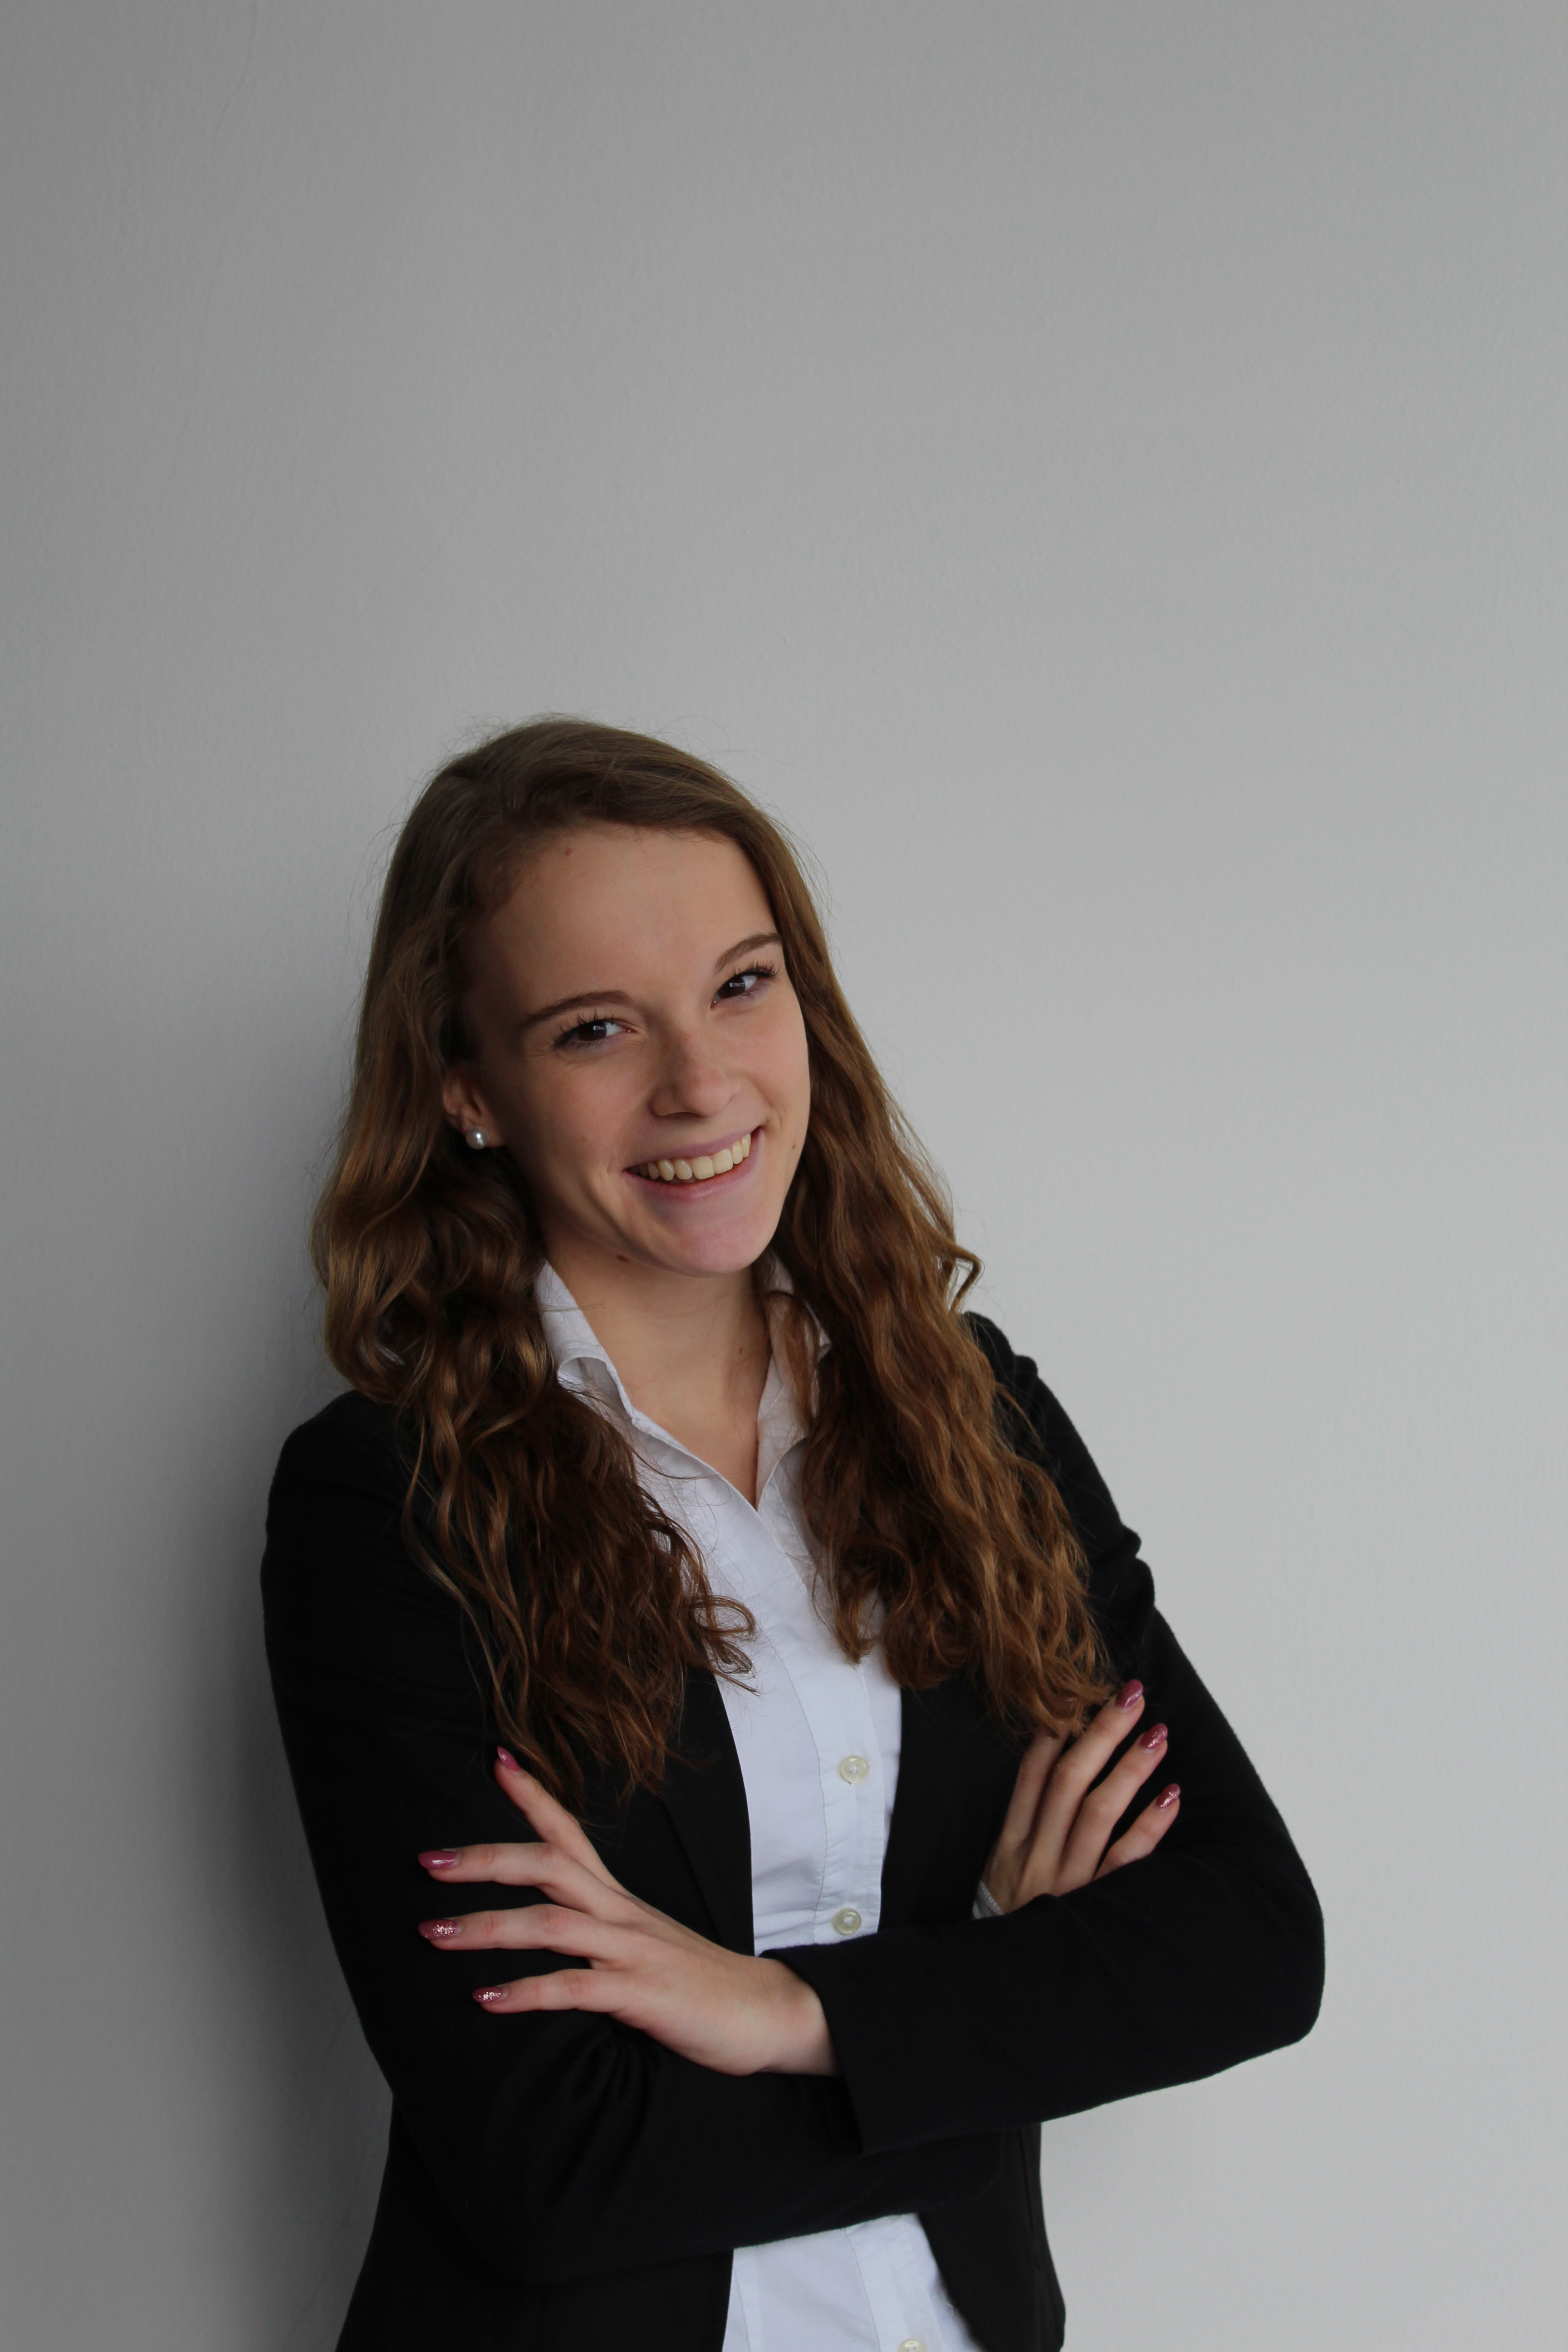
\includegraphics[width=0.3\textwidth] {bilder/Laura}
\end{wrapfigure}
\section*{Laura Rössl}
The role of the database expert was taken over by Laura who set up and maintained our database structure. She kept up with all the software structure changes and therefore changed the ERD on what we arranged beforehand. 

\begin{wrapfigure}{r}{0.3\textwidth}
    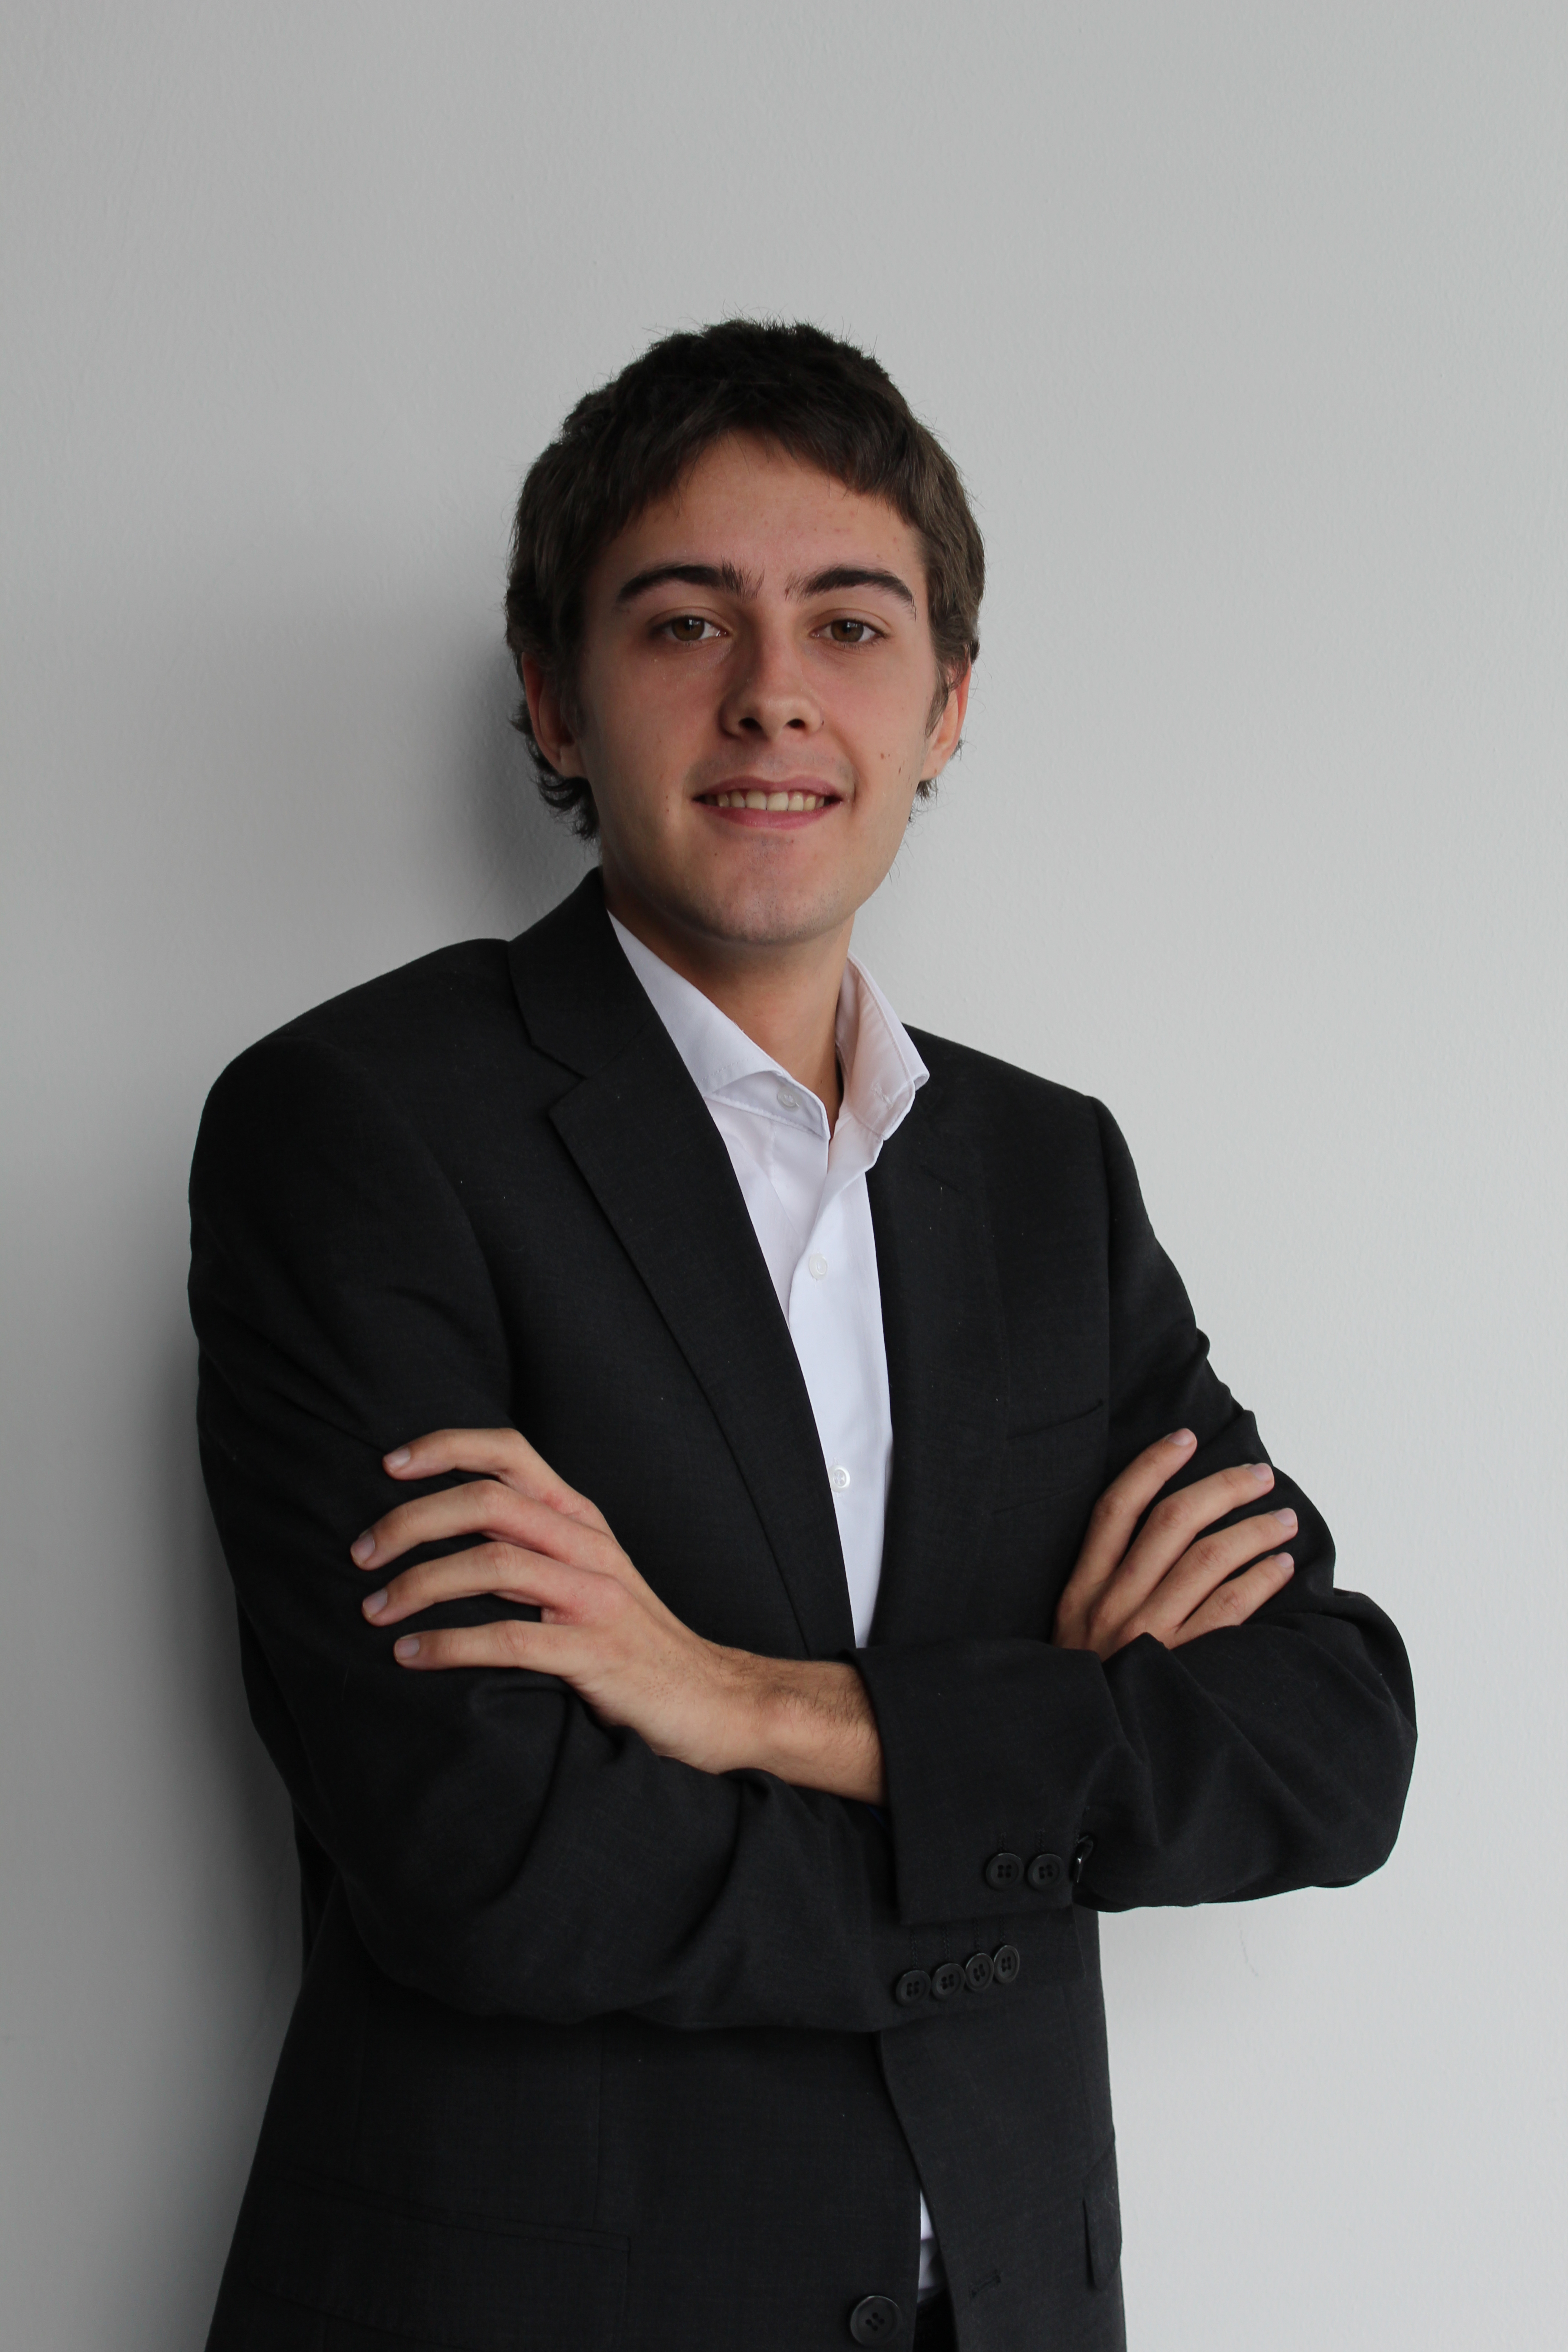
\includegraphics[width=0.3\textwidth] {bilder/Paul}
\end{wrapfigure}
\section*{Paul Zwölfer}
Paul's responsibility was the programming of the software for the working prototype. He provided a lot of technical information on software, modules and the different API's. Due to his engagement and never ending ambition, the development of the software went very well.

Together with Claudio, he started to test the software right from the first working state. This helped to avoid problems and provide a well conceived programme structure.
\chapter*{Statutory Declaration}
\addcontentsline{toc}{chapter}{Statutory Declaration}
With this I declare that all work presented in this diploma thesis is my own mindwork. I have used only the referred sources and aids and all parts which have been either literally or in general manner from other sources have been indicated accordingly.
\newline \newline
Furthermore, the secondary technical school HTBLA Kaindorf/Sulm is privileged to use any of my work included in this diploma thesis for educational or research purposes, as long as special attention is paid to data security and competitional regulations.
\par\bigskip

\par\bigskip

\par\bigskip

\par\bigskip

\par\bigskip

\par\bigskip

\par\bigskip

\par\bigskip

\par\bigskip

\par\bigskip

\par\bigskip

\par\bigskip

\rule{6cm}{0.4pt} \space \rule{6cm}{0.4pt} 

asdf

\include{chapters/tableofcontents}
\chapter*{Foreword from the Employer}
Kilometre allowance and the documentation of driven kilometres for the company are important todos for every self employed entrepreneur. The fact is that writing every business car ride into an excel sheet or manually into a car log book is really annoying. It would be much more convenient if a device in my business car logs every trip and I am able to define my car rides via a web portal afterwards. This was the idea behind “Log book” which we wanted to test drive with our friends at HTBLA Kaindorf/Sulm. Next to the hardware prototype it was also important to get an idea for a possible database solution. To understand the project better we provided a design proposal next to the hardware to sum up the first section of the project.

But more important than the final outcome of the project is to see how young people are able to come up with new and interesting ideas and dive into project related subtasks which have to be accomplished. It is also great to transfer some of the know-how we have worked out and to see how these ideas are adopted and developed for the project.

I am sure that every project member is able to take something from this diploma thesis and use it for their own future business life. I wish Helena, Laura, Claudio and Paul the very best for the final exams. You are going to rock the stage.

  Best,\newline
Dominik\newline\newline
DI Dominik Fuchshofer, BSc\newline
CEO/CTO at Sunlime IT Services GmbH\newline
February 2016

\newpage
\chapter*{Introduction}
\addcontentsline{toc}{chapter}{Introduction}
\section*{State of the Art}
Lalala state of the art text \gls{it} olalalal
\begin{minted}{Java}
System.out.println("lalala");1111
\end{minted}
lalallivrgbnwo \gls{it} jialwsg
\newpage
\section*{Role of the Company}
In this part of our diploma-thesis it is listed up what our employer, Sunlime IT Services, contributes to the work of the electronic logbook, which includes following areas:
\begin{itemize}
\item Hardware
\item Data transfer
\item Design requirements
\item Content requirements
\end{itemize}
The company provides the RPi2 with all the components like GPS Module or antenna to create a working hardware prototype for the logbook.

Secondly, at the data transfer, they will define when and over which portal the data has to be sent. Moreover, it should be apparent which user is transferring the data, so it can be dedicated online. It is also important to consider the user data when designing the database. Furthermore, a feature list has to be defined and integrated.
The web server for the portal is also provided and maintained from the company.
\newline \newline
An external service provider creates the design from the existing wireframing and Sunlime IT Services implements the technical aspects to it. The external service provider should also design a Logo, which will be shown in the web portal.

Thirdly, the company has to choose a “Mobile-first” approach to react to the width of each end device.

Then, the logbook should also work on smartphones. Therefore, Adobe PhoneGap should help to transact the program. The mobile application has to be designed one time only.
\newline \newline
Finally, the company is responsible for the security on the servers. It should not be possible to have access on a server as third person. Passwords are only allowed to get saved encrypted.
\newpage
\section*{Goals}
The goal of our diploma-thesis is to build a working hardware prototype, which records GPS data. A RPi2 with a GPS module, has to be put into a car, to track GPS data and transfers it to a REST (Representational State Transfer) interface. REST is responsible for uploading data into the database. Due to the fact that we need to upload the GPS data into our database, we have to store the data locally on the RPi2 if there is no internet connection. The program structure is described in our Software description section.
\newline \newline
For our partner company, information about the user and for the user the tracks have to be stored in the database. To illustrate the structure of the databases, an Entity-Relationship diagram (ER Diagram) got created and designed. Furthermore, the Data Definition Language (DDL) and the Data Manipulation Language (DML) resulted out of the ER diagram.
\newline \newline
The wireframing is the Front-End representation of our diploma thesis. It displays the user interface on our web portal and mobile application. A user-friendly design is the result of our wireframing.
\newline \newline
To get a unique product, the market needs to get analysed. Here, the competitors should get detected and compared in different attributes. For instance: costs, supported platforms, GPS, hardware etc. With this information, a diploma-thesis should be created which differs from other products. Furthermore, other intended uses of the hardware prototype should get noted down.
\newline \newline
Last but not least, the project management of the working packets has to be defined appropriate and documented.
\section*{Working Hours}

\chapter{Software Requirements}
\section{Intially}
\subsection{Data Transmission}
It has to be clear when a transmission takes place and which data it contains. The user who is getting tracked must be recorded for the \gls{db} too.
\subsection{Data Design}
Also the information about the users have to be stored in the \gls{db}. Furthermore, a list of features has to be defined and integrated. This serves to adapting extensions of products from the competitive analysis.
\subsection{Webserver}
The webserver is provided and maintained by the company Sunlime IT Services. The server is located in a data center in Vienna and is tethered with 10\gls{gbitps}.
\section{Additional Requirements}
\subsection{\gls{rest}}
We switched to the technology \gls{rest} to save data in the \gls{db}. Our \gls{rest} Server is written in \gls{php} and uploads data.
\subsection{MySQL Database}
Since our partner companies main products are homepages, they already had a running \gls{mysql} \gls{db}. So they created a new workspace for us, which we could use.
\chapter{Competitor Analysis}
\section{Introduction}
In this part of our diploma thesis we give you some information about our current competitors with who we are sharing our project idea.
\newline \newline
One important factor to create an outstanding product and to lead the market is to know our competitors. Like it is said “Keep your friends close, but your enemies closer”. So,  we were supposed to do some researches about similar products, which are listed on the next few pages. We try to sum up the most important facts and a short description of the products competing. 
\newline \newline
The competitor analysis showed us what we have to look at and what customers exactly need. 
\paragraph{Compared Products}
\begin{itemize}
\item Miles
\item OsmAnd
\item TOMTOM
\item Fahrtenbuch (von Stefan Meyer)
\item TOUR
\item Mileage Logbook
\item Fahrtenbuch (myLogbook)
\item MyLog GPS Fahrtenbuch Kosten
\item Carpanion
\item Fahrtenbuch Mileage Book
\item Trucker Logbook
\item Logbuch App
\item Drives Fahrtenbuch
\item Abax Triplog
\item GPS Log Book
\item GPS Log Book Live
\item Gurtam
\item Maxtech
\item Tractive
\end{itemize}
\newpage
\section{Miles}
\paragraph{Source} 
\paragraph{Costs} 10 \euro
\paragraph{Supported Platforms} The application Miles is compatible for IOS 8.
\paragraph{GPS} No GPS connection necessary.
\paragraph{Business/Private mode} You can split your private tracking from your business tracking.
\paragraph{Hardware} No Hardware. App is only used on smartphones.
\paragraph{Access Forms} App
\paragraph{Manual/Automatic Tracking} Data can only be entered manually.
\paragraph{Internet Connection} Internet connection necessary.
\paragraph{Export} It’s possible to export data to a PDF or CSV File.
\paragraph{Other Features} No other features included.
\newpage
\section{OsmAnd}
\paragraph{Source} 
\paragraph{Costs} 
\paragraph{Supported Platforms} For Android and iOS smartphones and tablets. Also runs on a wide array of Linux-based systems.
\paragraph{GPS} Navigation- and tracking  system in one.
\paragraph{Business/Private mode} Only private mode.
\paragraph{Hardware} No Hardware. App is only used on smartphones.
\paragraph{Access Forms} App
\paragraph{Manual/Automatic Tracking} automatic
\paragraph{Internet Connection} No Internet connection necessary.
\paragraph{Export} It’s possible to export data to a PDF or CSV File.
\paragraph{Other Features} download offline Maps, which get used for tracking and navigation
\newpage
\section{TOMTOM}
\paragraph{Source} 
\paragraph{Costs} 
\paragraph{Supported Platforms} For Android (2.3.3 or higher) and IOS (5.0 or higher).
\paragraph{GPS} GPS connection is necessary.
\paragraph{Business/Private mode} You can split your private tracking from your business tracking.
\paragraph{Hardware} No Hardware. App is only used on smartphones.
\paragraph{Access Forms} App
\paragraph{Manual/Automatic Tracking} No information
\paragraph{Internet Connection}No information
\paragraph{Export} It’s possible to export data to a PDF or CSV File.
\paragraph{Other Features} No other features included.
\newpage
\section{Fahrtenbuch (von Stefan Meyer)}
\paragraph{Source} 
\paragraph{Costs} 
\paragraph{Supported Platforms} IOS
\paragraph{GPS} GPS connection is necessary.
\paragraph{Business/Private mode} You can split your private tracking from your business tracking.
\paragraph{Hardware} No Hardware. App is only used on smartphones.
\paragraph{Access Forms} App for iPhone and Apple Watch
\paragraph{Manual/Automatic Tracking} manual and automatic
\paragraph{Internet Connection} Internet connection is necessary.
\paragraph{Export} It’s possible to export data to a PDF or CSV File.
\paragraph{Other Features} No other features included.
\newpage
\section{TOUR}
\paragraph{Source} 
\paragraph{Costs} 
\paragraph{Supported Platforms} IOS
\paragraph{GPS} GPS connection is necessary.
\paragraph{Business/Private mode} You can split your private tracking from your business tracking.
\paragraph{Hardware} No Hardware. App is only used on smartphones.
\paragraph{Access Forms} App
\paragraph{Manual/Automatic Tracking} automatic
\paragraph{Internet Connection} Internet connection is necessary.
\paragraph{Export} It’s possible to export a Tax Office conform file.
\paragraph{Other Features}Trips can be combined afterwards
\newpage
\section{Mileage Logbook}
\paragraph{Source} 
\paragraph{Costs} 
\paragraph{Supported Platforms} Android 
\paragraph{GPS} GPS connection is necessary.
\paragraph{Business/Private mode} You can split your private tracking from your business tracking.
\paragraph{Hardware} No Hardware. App is only used on smartphones.
\paragraph{Access Forms} App
\paragraph{Manual/Automatic Tracking} automatic
\paragraph{Internet Connection} No internet connection is necessary.
\paragraph{Export} It’s possible to export data to a HTML, Excel or CSV File.
\paragraph{Other Features} No other features included.
\newpage
\section{Fahrtenbuch (myLogbook)}
\paragraph{Source} 
\paragraph{Costs} 
\paragraph{Supported Platforms} Android 
\paragraph{GPS} GPS connection is necessary.
\paragraph{Business/Private mode} Only business mode.
\paragraph{Hardware} No Hardware. App is only used on smartphones.
\paragraph{Access Forms} App
\paragraph{Manual/Automatic Tracking} automatic
\paragraph{Internet Connection} No internet connection is necessary.
\paragraph{Export} It’s possible to export data to a HTML, XML, INtex, Euro-Fahrtenbuch, Fahrtenbuch Express, WISO Fahrtenbuch or CSV File.
\paragraph{Other Features} No other features included.
\newpage
\section{MyLog GPS Fahrtenbuch Kosten}
\paragraph{Source} 
\paragraph{Costs} 
\paragraph{Supported Platforms} Android
\paragraph{GPS} GPS connection is necessary.
\paragraph{Business/Private mode} You can split your private tracking from your business tracking.
\paragraph{Hardware} No Hardware. App is only used on smartphones.
\paragraph{Access Forms} App
\paragraph{Manual/Automatic Tracking} automatic
\paragraph{Internet Connection} No internet connection is necessary.
\paragraph{Export} It’s possible to export data to a PDF File.
\paragraph{Other Features} No other features included.
\newpage
\section{Carpanion}
\paragraph{Source} 
\paragraph{Costs} 
\paragraph{Supported Platforms} Android, IOS, Windows
\paragraph{GPS} GPS connection is necessary.
\paragraph{Business/Private mode} Only private mode.
\paragraph{Hardware} No Hardware. App is only used on smartphones.
\paragraph{Access Forms}Web Form and App
\paragraph{Manual/Automatic Tracking} manual
\paragraph{Internet Connection} Internet connection necessary.
\paragraph{Export} It’s possible to export data to a PDF or CSV File.
\paragraph{Other Features} You can take pictures of your fuel receipts and save them together with your refueling stops.
\newpage
\section{Fahrtenbuch Mileage Book}
\paragraph{Source} 
\paragraph{Costs} 
\paragraph{Supported Platforms} Android, IOS, Windows
\paragraph{GPS} GPS connection is necessary.
\paragraph{Business/Private mode} You can split your private tracking from your business tracking.
\paragraph{Hardware} No Hardware. App is only used on smartphones.
\paragraph{Access Forms} Web form, App
\paragraph{Manual/Automatic Tracking} automatic and manual
\paragraph{Internet Connection} No internet connection necessary.
\paragraph{Export} It’s possible to export data to a PDF, XML, Excel or CSV File.
\paragraph{Other Features} No other features included.
\newpage
\section{Trucker Logbook}
\paragraph{Source} 
\paragraph{Costs} 
\paragraph{Supported Platforms} Android, IOS
\paragraph{GPS} No information
\paragraph{Business/Private mode} Only business mode.
\paragraph{Hardware} No Hardware. App is only used on smartphones.
\paragraph{Access Forms}Web form, App
\paragraph{Manual/Automatic Tracking} manual
\paragraph{Internet Connection} No information
\paragraph{Export} No information
\paragraph{Other Features} No other features included.
\newpage
\section{Logbuch App}
\paragraph{Source} 
\paragraph{Costs} 
\paragraph{Supported Platforms} IOS
\paragraph{GPS} GPS connection is necessary.
\paragraph{Business/Private mode} Only private mode.
\paragraph{Hardware} No Hardware. App is only used on smartphones.
\paragraph{Access Forms} App
\paragraph{Manual/Automatic Tracking} No information
\paragraph{Internet Connection} No information
\paragraph{Export} It’s possible to export data to a PDF File, Excel or CSV File.
\paragraph{Other Features} Weather
\newpage
\section{Drives Fahrtenbuch}
\paragraph{Source} 
\paragraph{Costs} 
\paragraph{Supported Platforms} IOS
\paragraph{GPS} No information
\paragraph{Business/Private mode} You can split your private tracking from your business tracking.
\paragraph{Hardware} No Hardware. App is only used on smartphones.
\paragraph{Access Forms} App
\paragraph{Manual/Automatic Tracking} The manual tracking version is cost free, but at the chargeable version the automatic tracking is possible and you can split your private and business tracking.
\paragraph{Internet Connection} No information
\paragraph{Export} It’s possible to export data to a PDF or CSV File.
\paragraph{Other Features} 
\begin{itemize}
\item You can use database entries as pattern for future tracks
\item Statistics
\item Backups
\item In the chargeable version of the app, you can register more than one vehicle
\end{itemize}
\newpage
\section{Abax Triplog}
\paragraph{Source} 
\paragraph{Costs} 
\paragraph{Supported Platforms} 
\paragraph{GPS} 
\paragraph{Business/Private mode}
\paragraph{Hardware}
\paragraph{Access Forms}
\paragraph{Manual/Automatic Tracking}
\paragraph{Internet Connection}
\paragraph{Export}
\paragraph{Other Features}
\newpage
\section{GPS Log Book}
\paragraph{Source} 
\paragraph{Costs} 
\paragraph{Supported Platforms} 
\paragraph{GPS} 
\paragraph{Business/Private mode}
\paragraph{Hardware}
\paragraph{Access Forms}
\paragraph{Manual/Automatic Tracking}
\paragraph{Internet Connection}
\paragraph{Export}
\paragraph{Other Features}
\newpage
\section{GPS Log Book Live}
\paragraph{Source} 
\paragraph{Costs} 
\paragraph{Supported Platforms} 
\paragraph{GPS} 
\paragraph{Business/Private mode}
\paragraph{Hardware}
\paragraph{Access Forms}
\paragraph{Manual/Automatic Tracking}
\paragraph{Internet Connection}
\paragraph{Export}
\paragraph{Other Features}
\newpage
\section{Gurtam}
\paragraph{Source} 
\paragraph{Costs} 
\paragraph{Supported Platforms} 
\paragraph{GPS} 
\paragraph{Business/Private mode}
\paragraph{Hardware}
\paragraph{Access Forms}
\paragraph{Manual/Automatic Tracking}
\paragraph{Internet Connection}
\paragraph{Export}
\paragraph{Other Features}
\newpage
\section{Maxtech}
\paragraph{Source} 
\paragraph{Costs} 
\paragraph{Supported Platforms} 
\paragraph{GPS} 
\paragraph{Business/Private mode}
\paragraph{Hardware}
\paragraph{Access Forms}
\paragraph{Manual/Automatic Tracking}
\paragraph{Internet Connection}
\paragraph{Export}
\paragraph{Other Features}
\newpage
\section{Tractive}
\paragraph{Source} 
\paragraph{Costs} 
\paragraph{Supported Platforms} 
\paragraph{GPS} 
\paragraph{Business/Private mode}
\paragraph{Hardware}
\paragraph{Access Forms}
\paragraph{Manual/Automatic Tracking}
\paragraph{Internet Connection}
\paragraph{Export}
\paragraph{Other Features}


\chapter{Prototype}
\section{RPi2 Hardware}
\pageauthor{Paul Zwölfer}
\subsection{GPS Module}
The \gls{gps} module had to be soldered to the \gls{gpio} pins. We didn't trust our soldering skills and tried to avoid damage to the module. But it turned out that we needed a maximum of reliability for the connection and decided to solder A to B.\newline
\includegraphics[width=0.48\textwidth]{bilder/GPS}
\subsection{GPS Antenna}
We only used the internal \gls{gps} antenna for testing. Our problem was that it took really long to get a \gls{gps} signal every time we changed the location. With the external antenna it worked much quicker. In the final product an external antenna would not be necessary because the gps board remembers the last position and a position update is faster by orders of magnitude.\newline 
\includegraphics[width=0.48\textwidth]{bilder/Antenna}
\subsection{UMTS Stick}
The \gls{umts} stick is necessary for transmitting the data to the \gls{db}.\newline
\includegraphics[width=0.48\textwidth]{bilder/Medion_3}
\subsection{UPS}
If the engine of the car is switched off, the power supply of the \gls{rpi2} is interrupted. When the \gls{rpi2} gets power from the engine again, it has to do a system check and repair all files. Our final product will use an \gls{ups}. This \gls{ups} supplies our \gls{rpi2} with power even if the engine of the car is turned off. This eliminates the problem of data loss.\newline
\includegraphics[width=0.48\textwidth]{bilder/USV}
\newpage
\subsection{OS}
\subsubsection{Raspbian Wheezy}
When we started our diploma thesis the most common operation system was and still is Raspbian Wheezy. At the beginning we downloaded the image and wrote the .img file on the microSD Card. You always have to connect the \gls{rpi2} to a screen to start Raspbian Wheezy. There you have to configure things like the keyboard layout. You can also do that later with the sudo raspi-config command. After that you have to reboot the \gls{rpi2}.
Since we wanted to have a remote connection, we installed a \gls{tvnc} Server on the \gls{rpi2}. For this, we used the  
\begin{minted}{python}
	sudo apt-get install tightvncserver
\end{minted}
command.\newline
To connect the \gls{rpi2} via a \gls{tvnc} Client, we had to start the server with the 
\begin{minted}{python}
	tightvncserver
\end{minted}
command. Then the Server started on the Port 5901. For the connection establishment, we had to write the \gls{ip} address and the Port 5901 into the \gls{tvnc} Client. After that, we started to configure everything for the use of the \gls{gps} module.
\paragraph{GPS} \mbox{}\\
First we had to configure the communication between the \gls{rpi2} and the \gls{uart} pins on it. These \gls{uart} pins are \gls{gpio} 14 and 15.\newline
To stop the sending of the debug information, we had to edit the following file /boot/cmdline.txt with the 
\begin{minted}{python}
	sudo nano /boot/cmdline.txt
\end{minted}
command.\newline
There was one line within this text file and there the following text needed to be deleted
\begin{minted}{python}
	console=ttyAMA0,115200 kgdboc=ttyAMA0,115200
\end{minted}
Now it looked like this: 
\begin{minted}{python}
/dwc_otg.lpm_enable=0 console=tty1 root=/dev/mmcblk0p2 rootfstype=ext4 
elevator=deadline rootwait
\end{minted}
The \gls{rpi2} sends all terminal output over the external serial. To disable this behaviour, we had to edit the /etc/inittab file. We did this with the 
\begin{minted}{python}
	sudo nano /etc/inittab
\end{minted}
command.\newline
There we had to comment out the following line:
\begin{minted}{python}
#Spawn a getty on Raspberry Pi serial line
T0:23:respawn:/sbin/getty -L ttyAMA0 115200 vt100
\end{minted}
and after we did that, it looked like:
\begin{minted}{python}
#Spawn a getty on Raspberry Pi serial line
#T0:23:respawn:/sbin/getty -L ttyAMA0 115200 vt100
\end{minted}
An interesting thing was, that this file did not exist on the Raspbian Jessie Lite image. There we had to change nothing.\newline
The next step was to ensure if the Raspbian was up-to-date. At the beginning we did that with the 
\begin{minted}{python}
	sudo apt-get update
\end{minted}
and the 
\begin{minted}{python}
	sudo apt-get dist-upgrade
\end{minted}
command. Then we had to restart the \gls{rpi2}. We waited, but the \gls{rpi2} did not boot. So to find out what's going on, we connected the \gls{rpi2} to a screen and looked at the output. It showed us something like that all CPU stopped and at the end there was a line that looked like this:
\begin{minted}{python}
	---[ end Kernel panic - not syncing: VFS: Unable to mount root 
	   fs on unknown-block(0,0)
\end{minted}
So we looked up for another option and found out that we should  use the 
\begin{minted}{python}
	sudo rpi-update
\end{minted}
command before rebooting. Searching for a fitting solution, we found many possibilities we had to try until we found the right one for our problem. So we started the whole process of ensuring if the Raspbian was up-to-date all over again. Actually we did this many times, for every possible solution we found.\newline
So after we used the 
\begin{minted}{python}
	sudo rpi-update
\end{minted} 
command and rebooted the \gls{rpi2}, we could finally continue.\newline
Now we had to download and configure the required packages. We had to use the pps-tools and the libcap-dev. We did this with the 
\begin{minted}{python}
	sudo apt-get install pps-tools
\end{minted}
and the 
\begin{minted}{python}
	sudo apt-get install libcap-dev
\end{minted}
commands.\newline
After that we also had to install the \gls{gpsd} with the following command:
\begin{minted}{python}
	sudo apt-get install gpsd gpsd-clients python-gps
\end{minted}
The \gls{gpsd} presents us the data over a small server.\newline
Before we could start the \gls{gpsd}, we had to kill all the running \gls{gpsd}'s. We did that with the 
\begin{minted}{python}
	sudo killall gpsd 
\end{minted}
command. Finally we could start it and use it with the 
\begin{minted}{python}
	sudo gpsd /dev/ttyAMA0 -F /var/run/gpsd.sock -G
\end{minted}
command.
\paragraph{GPS Data} \mbox{}\\
We had to test if the \gls{gps} was working. There are many command line interfaces presenting you the data so you can see something.\newline
There ist the 
\begin{minted}{python}
	sudo cgps -s
\end{minted}
command that shows following output: \newline
\includegraphics[scale=0.7]{bilder/scr1}
\newline
then the
\begin{minted}{python}
	sudo xgps
\end{minted}
command where you can see this:\newline
\includegraphics[scale=0.9]{bilder/scr2}
\newline
and at last the 
\begin{minted}{python}
	sudo gpsmon
\end{minted}
command to see following information: \newline
\includegraphics[scale=0.7]{bilder/scr3}
\newline
Then we wanted to save the \gls{gps} Data on the \gls{rpi2}. We did this with the 
\begin{minted}{python}
	gpspipe -r | grep '^\$G' | tee test.nmea 
\end{minted}
command.
But since we could not use the \gls{nmea} format, we had to transform it into something like \gls{gpx} or \gls{kml}. For that we used the GPSBabel command line program. GPSBabel converts \gls{gps} data into other formats and saves it into a file. But firstly we had to install GPSBabel with the 
\begin{minted}{python}
	sudo apt-get install gpsbabel 
\end{minted}
command. We converted it into both, \gls{kml} and \gls{gpx} and for that we had to use the two following commands.
To get a KML file, we used:
\begin{minted}{python}
	gpsbabel -i nmea -f test.nmea -o kml -F test.kml
\end{minted}
To get a GPX file, we used:
\begin{minted}{python}
	gpsbabel -i nmea -f test3.nmea -o gpx -F test3.gpx
\end{minted}
\paragraph{Program} \mbox{}\\
After we applied these commands, we started programming. We all know the programming language JAVA the best, so we decided to use it for our software.  

We looked for an \gls{api} for JAVA and found one and a small test program with it. \newline
But we needed JAVA on the \gls{rpi2} to run a JAVA program. We wanted to use JAVA 8, but there was no real JAVA 8 \gls{jdk} for the \gls{rpi2}, so we had to use JAVA 7. We installed it with the following command:
\begin{minted}{python}
	sudo apt-get install oracle-java7-jdk
\end{minted}
You can read later everything about the program.

\paragraph{Auto boot} \mbox{}\\
While developing we started our program mostly from our own notebooks, but in the final product we wanted it to start automatically after booting for further use. For the final product everything has to start after booting anyway. So we edited the /etc/rc.local file with the 
\begin{minted}{python}
	sudo nano /etc/rc.local
\end{minted} 
command. At the last position we added the line
\begin{minted}{python}
	/home/pi/autostart.sh 
\end{minted} 
This means, that the autostart.sh, that was created by us, will be called upon when the \gls{rpi2} starts. Then we created the autostart.sh with the 
\begin{minted}{python}
	nano autostart.sh
\end{minted}
command. In in this file we wrote:
\begin{minted}{python}
	#!/bin/sh

	sudo killall gpsd
	sudo gpsd /dev/ttyAMA0 -F /var/run/gpsd.sock -G
\end{minted}
To make the script executable we had to use the following command:
\begin{minted}{python}
	chmod +x autostart.sh
\end{minted}
\paragraph{Problems} \mbox{}\\
Here we are going to explain some problems which appeared and did not mention before.\newline
Since we had a \gls{wlan} stick, we wanted the \gls{rpi2} to be connected with a router. We found out, that the /etc/network/interfaces file must be edited. This was done with the
\begin{minted}{python}
	sudo nano /etc/network/interfaces 
\end{minted}
command.\newline
At the beginning it looked like this:
\begin{minted}{python}
	auto lo
	iface lo inet loopback

	auto eth0
	allow-hotplug eth0
	iface eth0 inet dhcp

	auto wlan0
	allow-hotplug wlan0
	iface wlan0 inet manual
	wpa-conf /etc/wpa_supplicant/wpa_supplicant.conf

	auto wlan1
	allow-hotplug wlan1
	iface wlan1 inet manual
	wpa-conf /etc/wpa_supplicant/wpa_supplicant.conf
\end{minted}
Then we changed the \gls{wlan} interface.
\begin{minted}{python}
	auto wlan0
	allow-hotplug wlan0
	iface wlan0 inet dhcp
	wpa-ssid "linksys"
	wpa-psk "raspberry"
\end{minted}
This worked out quite well, but if the \gls{rpi2} started and there was no \gls{wlan}, the \gls{rpi2} did not accept \gls{lan} too.
\newpage
\subsubsection{RASPBIAN JESSIE LITE}
Jessie Lite is a command line \gls{os}. Our final product will run on this \gls{os}, because it's starting much faster than Raspbian Wheezy. Additionally, Raspbian Wheezy is no longer updated since 2015 and isn't able to be downloaded from the official site since February 2016.
\paragraph{Getting started} \mbox{}\\
At the beginning we downloaded the Raspbian Jessie Lite image and wrote the .img file on the microSD Card. There was the first problem. The old Raspbian Wheezy image set the partition size to the maximum while booting. With Jessie Lite we had to do that on our own. 

The next problem was that the ethernet interfaces \gls{ip} was set to manual. Wheezy had set it to auto. So, if we want to have internet access from the beginning, we had to edit the interface file (/etc/network/interfaces) before booting the \gls{rpi2}. Since we did it after the boot, too, we are going to describe how to do that later and there you can also see what we changed in this file.

The next step was to edit the boot file(/boot/cmdline.txt). When this was carried out, the \gls{gpsd} received data from the pins. We changed the same at the ethernet interface later. In this file was no difference when we did it. 
\newline \newline
Here we had to remove 
\begin{minted}{python}
	console=ttyAMA0,115200
\end{minted}
Then it looked like this: 
\begin{quote}
\begin{verbatim}
	dwc_otg.lpm_enable=0 console=tty1 root=/dev/mmcblk0p2 
	rootfstype=ext4 elevator=$
\end{verbatim}
\end{quote}
After these applied changes, we inserted the microSD Card into the \gls{rpi2} and plugged it in.
\paragraph{GPS Configuration} \mbox{}\\
If we would not configure the ethernet interfaces \gls{ip} to manual, we have to connect the \gls{rpi2} to a screen. Then we edited the interface file(/etc/network/interfaces). This can be done with the 
\begin{minted}{python}
	sudo nano /etc/network/interfaces
\end{minted}
command. \newline
In this file there is a line iface eth0 inet manual and instead of this line we had to write:
\begin{minted}{python}
	auto eth0
	allow-hotplug eth0
	iface eth0 inet auto
\end{minted}
Then we rebooted the \gls{rpi2} and accessed it over the \gls{lan}. \newline
If we had not done it before, we would have to edit the boot file(/boot/cmdline.txt) with the following command:
\begin{minted}{python}
	sudo nano /boot/cmdline.txt
\end{minted}
There we removed console=ttyAMA0,115200 from the first line.\newline
After that we checked if everything was up to date with the following two commands:
\begin{minted}{python}
	sudo apt-get update
	sudo apt-get dist-upgrade
\end{minted}
Next we had to install different programs to get the \gls{gps} data.\newline
First we installed pps tools with the 
\begin{minted}{python}
	sudo apt-get install pps-tools
\end{minted}
command, the libcap dev with the 
\begin{minted}{python}
	sudo apt-get install libcap-dev
\end{minted}
command, and then the \gls{gpsd} with the 
\begin{minted}{python}
	sudo apt-get install gpsd gpsd-clients python-gps
\end{minted}
command.\newline
Since our program is written in JAVA, we also had to install JAVA with the 
\begin{minted}{python}
	sudo apt-get install oracle-java7-jdk
\end{minted}
command.\newline
Some other changes we had to apply on the Jessie Lite image, were editing the \gls{gpsd} file. We edited it with this command:
\begin{minted}{python}
	sudo nano /etc/default/gpsd
\end{minted}
Below you can see the whole file with our changes. 
\begin{minted}{python}
	# Default settings for the gpsd init script and the 
	hotplug wrapper.

	# Start the gpsd daemon automatically at boot time
	START_DAEMON="true"

	# Use USB hotplugging to add new USB devices 
	automatically to the daemon
	USBAUTO="false"

	# Devices gpsd should collect to at boot time.
	# They need to be read/writeable, either by user gpsd 
	or the group dialout.
	DEVICES="/dev/ttyAMA0"

	# Other options you want to pass to gpsd
	GPSD_OPTIONS=""

	# Additionally:
	GPSD_SOCKET="/var/run/gpsd.sock"
\end{minted}
\paragraph{Copy program on RPi2} \mbox{}\\
Now we had to copy the program on the \gls{rpi2}. We wanted to do that via \gls{usb} stick. But there was the next problem. With the old Wheezy image we just connected the \gls{usb} stick. With the Jessie Lite image we had to mount the stick. We created a new folder called usb in the /mnt/ directory.
\begin{minted}{python}
	sudo mkdir usb
\end{minted}
Then we had to mount the \gls{usb} stick. We did this with the
\begin{minted}{python}
	sudo mount /dev/sda1 /mnt/usb/ -o uid=1000
\end{minted}
command. If we wanted to unplug the \gls{usb} stick we had to use the 
\begin{minted}{python}
	sudo umount /mnt/usb
\end{minted}
command.\newline
Then had to copy the .tar.gz file to /opt with the \begin{minted}{python}
	sudo cp gps.tar.gz /opt
\end{minted}
command. To extract it, we used the 
\begin{minted}{python}
	sudo tar xzvf gps.tar.gz
\end{minted}
command.\newline

\paragraph{Autostart(as Daemon)} \mbox{}\\
We created a gps\_rest.service script and put it into a folder near our program called systemd. Our script looks like this:
\begin{minted}{python}
	[Unit]
	Description=GPS Rest Daemon PaClLaHell
	[Service]
	ExecStart=/sbin/start-stop-daemon --start --quiet --make-pidfile 
	--pidfile /var/run/gps_rest.pid --background --user pi --chuid pi 
	--chdir /opt/gps --exec /usr/bin/java -- -jar GPS_REST.jar
	ExecStop=/sbin/start-stop-daemon --stop --quiet --pidfile 
	/var/run/gps_rest.pid --user pi --chuid pi --exec /usr/bin/java
	Type=forking
	[Install]
	WantedBy=multi-user.target
\end{minted}
%versteh den nächsten satz nicht
Then in /etc/systemd/system/multi-user.target.wants we create a like too the gps\_rest.service (\textit{sudo ln -s /opt/gps/systemd/gps\_rest.service}).
After that we rebooted the \gls{rpi2} and started the GPS\_REST.jar as a daemon.
To start and stop the daemon, we used following commands:
\begin{minted}{python}
	sudo systemctl start gps_rest.service
	sudo systemctl stop gps_rest.service
\end{minted}
And to get information about the daemon we used this command:
\begin{minted}{python}
	sudo systemctl status gps_rest.service
\end{minted}
\paragraph{UMTS Stick} \mbox{}\\
Since the \gls{umts} stick is not the newest, it was not that easy to make it working with the \gls{rpi2}.
\subparagraph{Configure the USB config} \mbox{}\\
At first we had to configure the \gls{rpi2} so it would accept the stick as a modem.\newline
We created a file in /opt/gps/udev and there we had to name this file 70-usb-modeswitch.rules. In this file we had to add this line:
\begin{minted}{python}
	ACTION=="add", SUBSYSTEM=="usb", 
	ATTRS{idVendor}=="0e8d", 
	ATTRS{idProduct}=="0002", 
	RUN+="/usr/sbin/usb_modeswitch -v 0e8d -p 0002 -M 
	'555342431234567800000000000006f0010300000000000000000000000000'"
\end{minted}
Then we had to create a link to the right position, that was /opt/gps/udev/rules/. This has been done with the 
\begin{minted}{python}
	sudo ln -s /opt/gps/udev/rules/70-usb-modeswitch.rules
\end{minted}
command.\newline
After that the following command showed us if the ID from the stick was right.
\begin{minted}{python}
	lsusb
\end{minted}
\subparagraph{Configuration of the provider}\mbox{}\\
To make configurations, we had to change to the super user state, with the 
\begin{minted}{python}
	sudo su
\end{minted}
command.\newline
After that we had to create two files with information for ppp. \newline
We created the first file called hot\_internet in /etc/chatscripts/. \newline
In this file we had to put these lines:
\begin{minted}{python}
	TIMEOUT 10
	ABORT 'BUSY'
	ABORT 'NO ANSWER'
	ABORT 'ERROR'
	ABORT 'NO CARRIER'
 
	'' 'ATZ'
	'OK' 'ATE1'
	'OK' 'AT+CGDCONT=1,"IP","webaut","0.0.0.0",0,0'
	'OK' 'ATDT*99#'
	'CONNECT' '\c'
\end{minted}
The next file was also called hot\_internet and created in /etc/ppp/peers/.\newline
This file looked like this:
\begin{minted}{python}
	hide-password
	noauth
	connect "/usr/sbin/chat -v -f /etc/chatscripts/hot_internet"
	debug
	/dev/ttyUSB0
	115200
	defaultroute
	replacedefaultroute
	noipdefault
	usepeerdns
	crtscts
	lock
	local
	 
	# Redial and interval
	persist
	holdoff 5
	 
	# No compression
	novj
	novjccomp
	nopcomp
	nodeflate
		 
	# PAP authentication
	 
	# LCP echo messages settings
	lcp-echo-failure 4
	lcp-echo-interval 65535
\end{minted}
After that we could start it with 
\begin{minted}{python}
	pon hot_internet
\end{minted}
and stop it with 
\begin{minted}{python}
	poff hot_internet
\end{minted}
\subparagraph{Auto boot PPP}\mbox{}\\
When pon/poff worked, we had to configure the /etc/network/interfaces and here we had to add the ppp interface as you can see in the following code lines:
\begin{minted}{python}
	# interfaces(5) file used by ifup(8) and ifdown(8)
	 
	# Please note that this file is written to be used with dhcpcd
	# For static IP, consult /etc/dhcpcd.conf and 'man dhcpcd.conf'
 
	# Include files from /etc/network/interfaces.d:
	source-directory /etc/network/interfaces.d
	 
	auto lo
	iface lo inet loopback
	 
	auto eth0
	iface eth0 inet dhcp
	 
	allow-hotplug ppp0
	auto ppp0
	iface ppp0 inet ppp
	provider hot_internet
	 
	allow-hotplug wlan0
	iface wlan0 inet manualrp
	    wpa-conf /etc/wpa_supplicant/wpa_supplicant.conf
	 
	allow-hotplug wlan1
	iface wlan1 inet manual
	    wpa-conf /etc/wpa_supplicant/wpa_supplicant.conf
\end{minted}
\textbf{References:} \cite{gpsd}, \cite{USBModeSwitch}, \cite{GSMmobile}, \cite{USBModemStickMedion}, \cite{PPPunderUbuntu}, \cite{USBSurfstick}, \cite{Reboot}, \cite{DaemonizeJavaApplications}, \cite{raspberrypi}, \cite{Tastaturlayout}, \cite{TightVNCServer}, \cite{RaspberryPiGPS}, \cite{gpsbable}, \cite{autostartScript}, \cite{wlan}
\clearpageauthor
\newpage
\section{Software Description}
\pageauthor{Laura Rössl}
The software of our \gls{rpi2} consists of two threads and a blocking FileObjectQueue. We get the \gls{gps} data from the \gls{api} and upload it via \gls{rest} in the \gls{db}. 
\subsection{Functions}
First of all a logging property file and a gps property file are loaded. The logging property file contains logging information like the saving location and the maximum number of logging files. The gps property file contains the raspberry id, the server \gls{url} and the gps module \gls{ip}.
\subsection{GPS API}
The \gls{api} (Gpsd4java) manages the connection with the \gls{gps} daemon, that covers receiving data, parsing this information into an useful format and supplying it to the “API Thread”. The \gls{gps} data we use consists of the timestamp, coordinateX, coordinateXError, coordinateY, coordinateYError, acceleration, altitude and altitudeError.
\subsection{Tape API}
We implemented this \gls{api}, because of the problem with saving data into an offline file. This \gls{api} provides us a FileObjectQueue where we can put and remove our points and this FileObjectQueue is automatically saved in a file. 
\subsection{Save Thread}
The Save thread reads point data from the FileObjectQueue and sends the data to the \gls{rest} server. When the tracks are written in the database, the Save Thread removes these points from the FileObjectQueue.
\subsection{API Thread}
When the GPS API measures \gls{gps} data, the API Thread gets it from the \gls{api}. The API Thread adds the information about the track and loads it into the FileObjectQueue.
\begin{center}
\includegraphics[width=1\textwidth]{bilder/SoftwareDiagram1}
\end{center} 
\subsection{PHP (REST)}
This part of our software is responsible for the upload into the database. The \gls{rest} server gets the data formatted as \gls{json}.
\begin{center}
\includegraphics[width=1\textwidth]{bilder/SoftwareDiagram2}
\end{center} 
\clearpageauthor
\section{Code Structure}
\pageauthor{Paul Zwölfer}
\subsection{Classes}
\subsubsection{GPS.java}
\paragraph{Constructor}\mbox{}\\
In the GPS.java class, the gpsModuleAddress variable is initialized and gets its value from the GPSConfiguration.java class.
\paragraph{startGpsdClient}\mbox{}\\
In the startGpsdClient method, the GPS API is initialized and the validate method from the BL.java class is called every time we get data from the GPS API.
\subsubsection{BL.java}
\paragraph{Constructor}\mbox{}\\
In this class the FileObjectQueue is created and initialized by the save.jPoint file and the GsonConverter.java class. 
Then a new track is created and at last the SaveDataThread object is initialized and started.
\paragraph{Validate}\mbox{}\\
Checks if the data from the GPS API is a number. If not it will be set to 0 except the latitude and the longitude. If they are \gls{nan} it will do nothing. 
Then it adds the data from the GPS API to the FileObjectQueue.
\paragraph{ProcessData}\mbox{}\\
This method peeks max 50 and min 15 points from the FileObjectQueue and puts them into a JContainer. Then it sends these points to the DataManager.java class to upload them via the uploadContainer method.
\subsubsection{SaveDataThread.java}
This is an intern Class in the \gls{bl} class that extends Thread.
\paragraph{Run}\mbox{}\\
This override method calls the ProcessData method and then waits 1 second.
\subsubsection{Data Manager.java}
\paragraph{Constructor}\mbox{}\\
Gets the server \gls{url} and puts it on the urlString variable.
\paragraph{UploadContainer}\mbox{}\\
Uploads the JContainer it got to the Server via \gls{rest} .
\subsubsection{JContainer.java}
This is a beans class that contains attributes, getter and setter methods for the respective attribute and a toString method of the JContainer.
\subsubsection{JPoint.java}
This is a beans class that contains attributes, getter and setter methods for the respective attribute and a toString method of the JPoint.
\subsubsection{GPSConfiguration.java}
At the beginning this class loads the logging properties.
\paragraph{InitConfiguration}\mbox{}\\
Reads the properties for the program from a file and sets these values on the specified variables. If a value is not in the file, it sets a default value. And at the end it closes the file.
\subsubsection{GsonConverter.java}
This class is a converter class that has implemented a FileObjectQueue Converter. In the method, the bytes from the file are converted, so that they can be saved on the FileObjectQueue. In the toStream method, it is the other way round, so the FileObjectQueue is saved on a file.
\subsection{Class Diagram}
\begin{center}
\includegraphics[width=1\textwidth]{bilder/GPS_REST_UML_Diagram}
\end{center}
\clearpageauthor
\section{Problems}
\pageauthor{Claudio Knapp}
\subsection{Uploading into Database}
When we started with this project, we uploaded tracked data directly into the database over a standard java database connection. Beside working on this project, we learned the technology hibernate in school so we reconstructed our program and used hibernate. Later our employer told us, that we should use \gls{rest} to upload data for a higher security level and fewer connections to the database and therefore less overhead. Another reason why we had to use this web service technology is that it's not possible to directly access the \gls{db} from outside. We wrote the \gls{rest} \gls{php} script on our own. 
\subsection{Offline Saving}
When the engine stopped while saving data offline, we had a loss of points, because the whole save file we used was overwritten. So we created a copy of this file, removed the data that was already in the database and deleted the original file. Then we renamed the copy to the original file name. Nevertheless, there was still a problem. On the one hand, it was possible that no data was lost, but on the other hand everything could be lost if the power was cut off between deleting the original file and renaming the copy. This is the reason why we use Tape API now. 
\section{Functional Testing}
To ensure functionality of the hardware prototype and the software, we had to do several tests. They reach from logical problems to practical testing on the road.
\subsection{Database Connection Error}
While developing our software, the error handling when loosing database connection was a very important issue. We had to think about different solutions for different code structure because we changed the database connection type several times. 
\newline \newline
We decided on the connection type called \gls{rest}. When using a technology that relies heavily on a working internet connection, there had to be a backup plan if exactly this connection is not working anymore.
\newline \newline
When does an connection error occur:
\begin{itemize}
\item internet not working
\item database not working/running
\end{itemize}
We decided on saving points, that cannot be uploaded, into a \gls{json} (save.jPoint). This solution proved to be the most fitting idea we thought of. It perfectly handled the described problems, reliably managed points and the saving mechanism worked phenomenal.
\newline \newline
The same concept is used when the database is offline or not working properly. 
\subsection{Inaccuracy of the GPS Coordinates}
After the first tests, where we tried to get \gls{gps} signal, we noticed a slight inaccuracy of the signal. This inaccuracy gets influenced by several factors. Therefore we had to find out how precise our \gls{gps} coordinates are and how much of an imprecision (part of the \gls{gps} data we get from our module) there is. 
\newline \newline
We evaluated driven tracks and measured how much distance there is between the actual location and the \gls{gps} coordinates received. This difference was about 5 metres, so no problem at all. 
\newline \newline
Due to the fact that we receive how much of an inaccuracy there is in the \gls{gps} data, our partner company can easily extract this information and compensate it in the visualization process. To do that even better, we also saved the deviation and the altitude.

\begin{center}
%grafiken der gefahrenen strecken --> claudio
%\includegraphics[width=1\textwidth]{}
\end{center}

\subsection{No GPS Signal}
When handling the \gls{gps} inaccuracy, we had to take into account that there could be no signal at all. Therefore we had to decide on a solution when receiving this data and how to handle and save it.
\newline \newline
We tried different solutions, but finally decided on not saving them. It is the most efficient way concerning storage, both offline and online.
\newline \newline
Meaning of not saving data when having no signal:
\begin{itemize}
\item when there is no \gls{gps} signal, there is often also no internet connection
\item this leads to offline stored “null” points
	\begin{itemize}
	\item not saving these null points is the best solution
	\end{itemize}		
\item data extraction for our partner company when displaying the data on maps will be easier
\end{itemize}
\textbf{References:}  \cite{Git}, \cite{Gpsd4java}
\clearpageauthor
\newpage
\section{Future Work and Ideas}
\pageauthor{Claudio Knapp}
Due to our limitation in time, we cannot infinitely improve our program. Therefore we sum up our future ideas on what could be implemented or improved. Of course, we only write about the things that came up to our minds, and therefore this is just a small list.
\paragraph{Security between RPi2 and REST service}\mbox{}\\
As we found out during the implementation process, \gls{rest} supports an encryption process. After consulting the partner company, we decided on not using the encryption on the prototype.
\paragraph{Access via SSH over UMTS}\mbox{}\\
It should be possible to access the \gls{rpi2} over the internet via \gls{ssh} for remote maintenance.
\paragraph{Critical error reporting}\mbox{}\\
If a severe problem happens, \gls{rpi2} should be able to report that problem so that it can be fixed.
\paragraph{Mobile Application/Webform}\mbox{}\\
Using the wireframing of the webform and mobile devices, it is possible to create an access interface that can be accessed via a web browser or a mobile application.
\paragraph{Putting the GPS Points on the street}\mbox{}\\
As shown in the Functional Testing part, the \gls{gps} data is rather inaccurate. Therefore our partner company has to interpolate and/or use the inaccuracy we add to the uploaded data. This task was not possible not accomplish in the given time, but could be implemented afterwards.

Compensating the inaccuracy will help to get an exact distance measurement and provide a better user experience.
\paragraph{Optimize Http overhead}\mbox{}\\
If there are many points on the \gls{rpi2}  and the connection is established, the connection should only be closed after sending all the Points.
\clearpageauthor
\chapter{Database}
One of our four main parts of our diploma thesis was the data design and \gls{db}. We started with creating an entity relationship diagram. This \gls{erd} was the base of our \gls{db}. Because of constant changes in our program structure, we had to change the \gls{db} structure too. 
\section{Entity Relationship Diagram}
\begin{center}
\includegraphics[width=0.9\textwidth]{bilder/ERD_new}
\end{center} 
Customer(svnr, firstname, lastname, dateofbirth, addressIDFK)\newline
Vehicle(vehicleID, svnrFK)\newline
Address(addressID, street, zipcode)\newline
TrackingHardware(serialNumber, svnrFK, description, licenceIDFK)\newline
Licence(licenceID, svnrFK, dateofactivation)\newline
Track(id, serialNumberFK, timestamp)\newline
Point(id, timestamp, (track\_id,track\_serialNumber)FK ,coordinateX, coordinateXError, coordinateY, coordinateYError, acceleration, altitude, altitudeError, distance)\newline
Vehicle\_TrackingHardware(serialNumberFK, vehicleIDFK)
\section{Entities}
\subsection{Customer}
The entity Customer has the social security number as the primary key. Additional attributes are the firstname, the lastname and the date of birth of the person the account belongs to. As you can see in the \gls{erd}, every customer has one reported address and an address can belong to zero or more customers. Due to this, the entity customer contains a foreign key with the id from the address. A customer can only register once, so every customer can have zero or one AdministrationAccount, depending on if he is already registered. Clearly, an account can only belong to one customer so it is well defined who is the owner of the device. There can be a customer who drives more than one vehicle so if he changes to another car, of course he does not have to buy a new device. He can use it for zero or more vehicles. The vehicle is only reported for one customer. This is because if the car is used by more than one person they will not have more than one account. Even if a customer usually only needs one device, it is possible for him to buy zero or more devices. And clearly he does not have to create a new administration account for each of them. But the other way around, every tracking hardware belongs to only one customer.
\subsection{Vehicle}
Every Vehicle has its own unique vehicle id to identify it. This id is also used in our \gls{db} to identify different vehicles. The vehicle is only reported for one customer. This is because if the car is used by more than one person they will not have more than one account. In one vehicle you can place zero or more tracking hardwares and one tracking hardware can be used in zero or more vehicles too, so this is called a “n to m relationship”. We splitted this relationship to an extra entity called Vehicle\_TrackingHardware. This entity contains the two primary keys of the first two tables as primary and foreign key at once.
\subsection{Address}
The entity Address has the unique address id for primary key to identify. It also contains the street name and the zipcode of each address. As you can see in the diagram, one address can belong to zero or more customers but one customer can only be reported to one address.
\subsection{TrackingHardware}
In our \gls{db}, every TrackingHardware is identified by its unique serial number. An additional attribute in this table is the description of the device. One hardware can only belong to one customer and one customer can own zero or more tracking hardwares. So we had to create a foreign key called svnr of the social security number of the Customer. Because of the already mentioned “n to m relationship” between TrackingHardware and Vehicle, you can see an extra entity called Vehicle\_TrackingHardware. With every purchase on a tracking hardware, you acquire an associated Licence. So this table includes the primary key of the Licence called licenceID as a foreign key. A Licence can belong to zero or one device. If the \gls{rpi2} is not purchased yet, the licence is not used. One TrackingHardware has already tracked zero or more Tracks and one Track always belongs to exactly one device.
\subsection{Licence}
The table Licence consists of its own unique licenceID. The svnr is the connection to the Customer Table and is a foreign key in this table. The Licence belongs to one Customer and the Customer can have zero and more Licences. The dateofactivation attribute is, as the names says, the date when the licence was activated on the web portal with the associated device.
\subsection{Track}
Every Track belongs to one TrackingHardware. This Track contains all the Points which belong to this Track. The identifier for the Track is a \gls{uuid}, generated by the program on the \gls{rpi2} and the serialNumber from the TrackingHardware. The table also has a timestamp generated at the start of the program on the \gls{rpi2}.
\subsection{Point}
The greatest part of the information is stored in the Point table. There the identifier is also a \gls{uuid}, generated by the program on the \gls{rpi2}. The primary key is compound of the id, and the primary key from the Track table which is also the foreign key in the Point Table. The identifier from Track is composed of the tack\_id and the serialNumber. The other attributes are the coordinates, the variance of the coordinates, the acceleration, the altitude and the variance of the altitude. The last thing is the distance, which is empty at the time being. Every Point belongs to one Track and every Track contains zero or more points.
\section{Data Definition Language}
\begin{minted}{SQL}
CREATE TABLE Address(
addressID INT(6) AUTO_INCREMENT PRIMARY KEY,
street VARCHAR(30),
zipcode INT(6)
);
CREATE TABLE Customer(
svnr INT(6) PRIMARY KEY,
firstname VARCHAR(30) NOT NULL,
lastname VARCHAR(30) NOT NULL,
email VARCHAR(50) NOT NULL,
dateofbirth DATE NOT NULL,
addressID INT(6),
FOREIGN KEY fk_Customer(addressID)
REFERENCES Address(addressID)
);

CREATE TABLE Vehicle(
vehicleID INT(8) AUTO_INCREMENT PRIMARY KEY,
svnr INT(6),
FOREIGN KEY fk_Vehicle(svnr)
REFERENCES Customer(svnr)
);

CREATE TABLE Licence(
licenceID INT(8) AUTO_INCREMENT PRIMARY KEY,
svnr INT(6),
dateofactivation DATE NOT NULL,
FOREIGN KEY fk_account (accountID)
REFERENCES AdministrationAccount(accountID)
);

CREATE TABLE TrackingHardware(
serialNumber INT(8) AUTO_INCREMENT PRIMARY KEY,
svnr INT(6),
description VARCHAR(100),
licenceID INT(8),
FOREIGN KEY fk_trackHardw(svnr)
REFERENCES Customer(svnr),
FOREIGN KEY fk_licence(licenceID)
REFERENCES Licence(licenceID)
);

CREATE TABLE VehicleTrackingHardware(
serialNumber INT(8),
vehicleID INT(8),
timestamp DATE NOT NULL,
PRIMARY KEY (serialNumber, vehicleID),
FOREIGN KEY fk_vth_serialNumber(serialNumber)
REFERENCES TrackingHardware(serialNumber),
FOREIGN KEY fk_vth_vehicleID(vehicleID)
REFERENCES Vehicle(vehicleID)
);

CREATE TABLE Track(
id VARCHAR(255),
serialNumber INT(8),
timestamp BIGINT NOT NULL,
PRIMARY KEY(id, serialNumber),
FOREIGN KEY fk_track_serial(serialNumber)
REFERENCES TrackingHardware(serialNumber)
);

CREATE TABLE Point(
id VARCHAR(255),
timestamp BIGINT NOT NULL,
track_serialNumber INT(8),
track_id VARCHAR(255),
coordinateY DOUBLE NOT NULL,
coordinateYError DOUBLE NOT NULL,
coordinateX DOUBLE NOT NULL,
coordinateXError DOUBLE NOT NULL,
acceleration DOUBLE NOT NULL,
altitude DOUBLE NOT NULL,
altitudeError DOUBLE NOT NULL,
distance DOUBLE,
PRIMARY KEY(id, timestamp, track_serialNumber,track_id),
FOREIGN KEY fk_point_track(track_serialNumber, track_id)
REFERENCES Track(serialNumber, id)
);
\end{minted}
\section{Data Manipulation Language}
\begin{minted}{SQL}
INSERT INTO Address(addressID, street, zipcode)
VALUES(1,'Blumenweg',8430);
INSERT INTO Customer(svnr, firstname, lastname, email, dateofbirth, addressID)
VALUES(4523, 'Karl', 'Huber', 'karl.huber@gmail.com',
DATE_FORMAT('1970-12-09','%Y-%m-%d'),1);
INSERT INTO Vehicle(vehicleID, svnr)
VALUES(832,4523);
INSERT INTO Licence(licenceID, svnr, dateofactivation)
VALUES(832495,4523,DATE_FORMAT('2016-01-20','%Y-%m-%d'));
INSERT INTO TrackingHardware(serialNumber, description, licenceID)
VALUES(1234, 'Karlis Raspi', 832495);
INSERT INTO VehicleTrackingHardware(serialNumber, vehicleID, timestamp)
VALUES(1234, 832, DATE_FORMAT('2016-01-24','%Y-%m-%d'));
INSERT INTO Track ('id', 'serialNumber', 'timestamp') 
VALUES('018f8ff5-395b-42d2-b2f6-5c976292cd5e', 1234, 1455535245172);
INSERT INTO Point ('id', 'timestamp', 'track_serialNumber', 'track_id', 
'coordinateY', 'coordinateYError', 'coordinateX', 'coordinateXError', 
'acceleration', 'altitude', 'altitudeError', 'distance') 
VALUES('007dae03-c915-4aae-baf9-2b7c42a41e43', 1455535245172, 1234, 
'1f114f58-fd0c-4da6-a1b6-571ae9e79748', 46.78029, 14.815, 15.54794, 10.697, 
0.103, 277.3, 18.17, 0),
('dedc843e-e29b-4a0d-b32d-20cb718088ea', 1455535282394, 1234, 
'1f114f58-fd0c-4da6-a1b6-571ae9e79748', 46.780401667, 14.815, 15.547526667, 
10.697, 7.562, 279, 16.56, 0);
\end{minted}
\section{Problems}
While we tried to insert testing data into our \gls{db}, we noticed that it wasn’t possible to save the timestamp as milliseconds. After researches, we discovered that the problem was the version of our \gls{mysql} \gls{db} (version 5.5.46). Due to this problem we had to change the datatype of our timestamp into bigint.
\chapter{Wireframing}
\pageauthor{Laura Rössl, Paul Zwölfer}
\section{Smartphone}
The design for the smartphone consists of four different pages. 
\subsection{Login}
The login dialogue is the first page you see. There are two input fields; for the username and the password. Below these input fields there is the login button to confirm and login. Then there is a check box to stay logged in.

The link if the password has been forgotten and a button to register and create a new user account are the last things on this page.
\subsection{Menu}
The menu pops up from the left edge as you can see on the picture down below. It can be chosen between viewing the tracks, customize settings, view statistics and logout.
\subsection{Tracks}
On the tracks page a map shows the last track by default but on the bottom any available track can be chosen to view it.
\subsection{Settings}
Under settings, basically changes like edit the mail address or change the password of the account can be applied, but also if the default track type should be private or public.
\subsection{Statistics}
It’s possible to view a graph where information of driven tracks are shown. Every registered car of this account can be chosen to view its graph and additionally, it’s selectable if the displayed data was tracked within the last week, month or year.
\begin{center}
\includegraphics[width=0.4\textwidth]{bilder/Smartphone}
\end{center}
\section{Tablet}
The wireframing we created for the Tablet design is nearly similar to the smartphone design. Except of a few extensions, such as for renaming the device and editing tracks more precisely.
\subsection{Login}
The login dialogue is the first page you see. There are two input fields for the username and the password. Below these input fields there is the login button to confirm. Then there is a check box to stay logged in.
The link if the password has been forgotten and a button to register and create a new user account are the last things on this page.
\subsection{Menu}
The menu pops up from the left edge as you can see on the picture. It can be chosen between viewing the tracks, customizing settings, viewing statistics, renaming the device, registering a car and a logout.
\subsection{Tracks}
On the tracks page a map shows the last track by default. A track can be selected and there is the option to edit or merge a route.
\subsection{Settings}
Under settings, basic changes like editing the mail address or changing the password of the account can be applied, but also if the default track type should be private or public.
\subsection{Renaming Devices}
The \gls{rpi2} gets a random identification name from the start. It is possible edit this name if the user wishes so.
\subsection{Registering Car}
Over the account settings, it is possible to registrate a new car with your licence.
\subsection{Statistics}
It’s possible to view a graph where information of driven tracks is shown. Every registered car of this account can be chosen to view its graph and additionally, it’s selectable if the displayed data was tracked within the last week, month or year.
\begin{center}
\includegraphics[width=0.625\textwidth]{bilder/Tablet}
\end{center}
\section{Web Portal}
\subsection{Home}
Before the user is logged in, information about the product is shown on this page.

After the login, all tracks are shown and it is possible to change the tracks from private to public.
\subsection{Login}
The login dialogue is the first page you see. There are two input fields for the username and the password. Below these input fields there is the login button to confirm and login. Then there is a check box to stay logged in.
The link if the password has been forgotten and a button to register and create a new user account are the last things on this page.
\subsection{Settings}
Under settings, basic changes like editing the mail address or changing the password of the account can be applied, but also if the default track type should be private or public.
\subsubsection{Registering Car}
Over the account settings, it is possible to registrate a new car with your licence.
\subsubsection{Renaming Device}
The \gls{rpi2} gets a random identification name from the start. It is possible edit this name if the user wishes so.
\subsection{Track}
On the tracks page a map shows the last track by default. It can be chosen between the cars and the tracks of the respective cars can be viewed.
\subsubsection{Edit}
If a track is selected, there is the possibility of editing it. If the route isn’t complete or must be changed in any way, it can be done over the web portal. Should it happen that one track is splitted up into two or more tracks because of complications, you can merge them into one whole route.
\subsubsection{Create}
Here a new track can be created manually over the web portal and the route of the track can be chosen. It’s possible to set the start and end position of the new track and changing the route by pulling the line to the desired way.
\subsection{Statistics}
It’s possible to view a graph where information of driven tracks are shown. Every registered car of this account can be chosen to view its graph and additionally, it’s selectable if the displayed data was tracked within the last week, month or year.
\subsection{Menu}
The menu from the homepage contain home, tracks, statistics, settings and login. The menu item tracks contains subitems called edit and create. The subitems of settings are register car and rename device.

\begin{center}
\includegraphics[width=1\textwidth]{bilder/WebPortal}
\end{center}
\clearpageauthor
\chapter{Optional Uses}
\pageauthor{Laura Rössl}
The basic concept of our product was to track driven distances of a car you use for private and business purposes. Nevertheless, we thought about other possible uses for this product.
\section{Taxi}
One of our ideas for optional uses was for a taxi company. Our product could be placed in the taxi, the taxi driver presses a button if a new customer enters the car and the device calculates the price of the taxi ride based on the distance, the velocity and the fix basic costs. 
\section{Car Renting}
A car renting company usually gets paid for renting their cars per day. Our product could help them to control the use of their cars. Our product could track the distances the customer took so the company could calculate a suitable price. 
\section{Train Controller}
We thought about the optional use as a train controller for checking the current location of a train, check for complications and preventing delays. It would be also possible planning ahead to avoid incidents and more delays.
\section{Mowing Machine}
There are already mowing machines that can drive around in your garden on their own and they are already able to discover the shape of your ground. Using our product, you could extend the conventional device so you can choose between predetermined tracks that your mowing machine could take. It would also be possible to control your mowing machine over a mobile application to change the direction or stop mowing.
\section{Helicopter}
Another optional use for our product could be a controlling device for a helicopter. Choosing a flying track or checking the position and the track of the helicopter could be possible.
\section{Pet Tracking}
Another possibility for our product is to power the device with an battery pack and use it to track your pet. For example if you have a dog or a cat, you can put it on their collar for example and watch where it is and where it goes.
\begin{center}
\includegraphics[width=0.85\textwidth]{bilder/UseCase}
\end{center}
\clearpageauthor
\chapter{User Manual}
\section{General}
First of all, thank you for buying our product. With your purchase on our product, you acquired a licence. Now you can register on our web portal and create your own account. Using your purchased licence, you can activate the product and connect it with your user account. You can also transfer the product with the related licence to another user account. Over the web portal, you can log in and view tracks, visualize them and eventually edit them.
\section{Installation Regulations}
The product has to be placed in the car and connected with the cigarette lighter receptacle to get power. When starting the engine of the vehicle, the device powers itself up and starts searching for a GPS signal.
\section{LEDs}
When you connect the product to a power source you will see some LEDs light up.
There are three LEDs. A red one on top of the RPi2, which is for GPS module and two on the opposite side of the USB ports which are red and green.
When the red LED next to the green one is on, the RPi2 gets power.
The green LED on the RPi2 lights up when the device boots and prepares itself for tracking. When it is ready and it receives data it flickers quick.
And if the red LED on the RPi2 GPS module blinks once per second, it has a GPS signal
\section{Warnings}
\begin{itemize}
\item This product shall only be connected to an external power supply rated at 5V dc, and a minimum current of 500-700mA for model A and 700-1200mA for model B. Any external power supply used with the RPi2 shall comply with relevant regulations and standards applicable in the country of intended use. 
\item This product should not be overclocked as this may make certain components very hot. 
\item This product should be operated in a well ventilated environment and the case should not be covered. 
\item This product should be placed on a stable, flat, non-conductive surface in use and should not be contacted by conductive items. 
\item The connection of unapproved devices to the GPIO connector may affect compliance or result in damage to the unit and invalidate the warranty. 
\item All peripherals used with the RPi2 should comply with relevant standards for the country of use and be marked accordingly to ensure that safety and performance requirements are met. These articles include but are not limited to keyboards, monitors, and mice used in conjunction with the RPi2.
\item Where peripherals are connected that do not include the cable or connector, the used cable or connector has to offer adequate insulation and operation in order that the requirements of the relevant performance and safety requirements are met.
\end{itemize}
\paragraph{To avoid malfunction or damage to your device please observe following:}
\begin{itemize}
\item Do not expose it to water, moisture or place on a conductive surface whilst in operation.
\item Do not expose it to heat from any source; the RPi2 is designed for reliable operation at normal ambient room temperatures.
\item Take care whilst handling to avoid mechanical or electrical damage to the printed circuit board and connectors.
\item Avoid handling the printed circuit board while it is powered. Only handle by the edges to minimise the risk of electrostatic discharge damage.
\item The RPi2 is not designed to be powered from a USB port of the other connected equipment. If this is attempted, it may malfunction.
\end{itemize}




\chapter{Future Work and Ideas}
Due to our limitation in time, we cannot infinitely improve our program. Therefore we sum up our future ideas on what could be implemented or improved. Of course, we only write about the things which came up in our minds, and therefore this is just a small list.
\newline \newline
\textbf{\textit{Security between \gls{rpi2} and \gls{rest} service}} \newline
As we found out during the implementation process, \gls{rest} supports an encryption process. After consulting the partner company, we decided on not using the encryption on the prototype.
\newline \newline
\textbf{\textit{Access via \gls{ssh} over \gls{umts}}}
\newline
It should be possible to access the \gls{rpi2} over the internet via \gls{ssh} for remote maintenance.
\newline \newline
\textbf{\textit{Critical error reporting}}
\newline
If a severe problem happens, \gls{rpi2} should be able to report that problem so that it can be fixed.
\newline \newline
\textbf{\textit{Mobile Application/Webform}}
\newline
Using the wireframing of the webform and mobile devices, it is possible to create an access interface which can be accessed via a web browser or a mobile application.
\newline \newline
\textbf{\textit{Putting the \gls{gps} Points on the street}}
\newline
As shown in the Functional Testing part, the \gls{gps} data is rather inaccurate. Therefore our partner company has to interpolate and/or use the inaccuracy we add to the uploaded data. This task was not possible not accomplish in the given time, but could be implemented afterwards.

Compensating the inaccuracy will help to get an exact distance measurement and provide a better user experience.
\newline \newline
\textbf{\textit{Optimize Http overhead}}
\newline
If there are many points on the \gls{rpi2}  and the connection is established, the connection should only be closed after sending all the Points.

\chapter{Tools and Technologies}
\pageauthor{Claudio Knapp}
\begin{wrapfigure}{r}{0.2\textwidth}
  \begin{center}
    \includegraphics[width=0.2\textwidth] {bilder/java}
  \end{center}
\end{wrapfigure}
\section{Java}
We decided on using JAVA, because it runs on every platform, is easy to implement and our partner company could use it on Android devices too. Also the fact that every member of the group got 5 years of programming experience in this language, shows that it is the most fitting choice for us.

\section{TAPE API}
We implemented this \gls{api}, because of the problem with saving data into an offline file. This \gls{api} provides us a FileObjectQueue where we can put and remove our points. This FileObjectQueue is automatically saved in a file.

\section{GPS API}
This \gls{api} was rather hard to find because there are few possible ways of handling the \gls{gps} data from an \gls{rpi2} in JAVA. Nevertheless, we read through the excellent documentation and found ways to use this \gls{api} in an easy way.

\newpage
\section{RASPBIAN}
\begin{wrapfigure}{r}{0.2\textwidth}
  \begin{center}
    \includegraphics[width=0.2\textwidth] {bilder/raspbian}
  \end{center}
\end{wrapfigure}
As we tried out different things in linux on the Raspbian Wheezy during our NVSU lessons, it showed its potential. Another point why we used it, was that it was constructed to work perfectly with the \gls{rpi2}. Therefore, our first choice was this image for our \gls{rpi2}. Later we found out, that Raspbian Wheezy was not supported any more and so we had to switch to Raspbian Jessie Lite. Raspbian Jessie Lite is only a command line \gls{os}, so it is perfect for our project.
\section{GIT}
\begin{wrapfigure}{r}{0.2\textwidth}
  \begin{center}
    \includegraphics[width=0.2\textwidth] {bilder/git}
  \end{center}
\end{wrapfigure}
When working in a group, a good collaboration tool is needed. Our choice was GIT because we only made negative experiences.

Unfortunately, we had problems at the beginning of our software development. Everytime we tried to "PULL" committed changes, we encountered a merge conflict. This conflict somehow followed us throughout the whole development phase.

At the end, we also used GIT for LaTeX cooperation. Due to the usage of the GIT console, it was a very pleasant experience.
\begin{wrapfigure}{r}{0.2\textwidth}
  \begin{center}
    \includegraphics[width=0.2\textwidth] {bilder/googledrive}
  \end{center}
\end{wrapfigure}
\section{Google Drive}
At the beginning and almost through the whole project, we used Google Drive for document management, time reporting and organization.
The main Google products we have used were Google Docs and Google Tables.

Collaborating was the main reason why we used especially this technologies. It worked trouble-free and had option to restore older versions of documents, which came in handy from time to time.
\clearpageauthor
\section{PHP}
\pageauthor{Helena Adam}
\begin{wrapfigure}{r}{0.2\textwidth}
  \begin{center}
    \includegraphics[width=0.2\textwidth] {bilder/php}
  \end{center}
\end{wrapfigure}
Originally it stood for Personal Home Page, but now for recursive backronym. It was designed for web development, but also used as programming language. 

The usage of \gls{php} is based on \gls{rest}. It's functioning kind of like a server, which connects to the \gls{db}, uploads the \gls{gps} data and disconnects.
\section{BalsamiQ}
\begin{wrapfigure}{r}{0.2\textwidth}
  \begin{center}
    \includegraphics[width=0.2\textwidth] {bilder/balsamiq}
  \end{center}
\end{wrapfigure}
We used this tool to provide our wireframing plans and mock ups, since it is a rapid wireframing tool. Mockups make it simple to generate ideas for designs and to pick the best one. It was recommended and provided by our employer because they have made a very good experience when using it. Also we made a great experience with it. It was easy to handle and our ideas could be implemented fast. Moreover, it was apparent if the design is right for the  user experience or rather not.
\begin{wrapfigure}{r}{0.2\textwidth}
  \begin{center}
    \includegraphics[width=0.2\textwidth] {bilder/MySQL}
  \end{center}
\end{wrapfigure}
\section{MySQL}
Our employers standard as database technology was \gls{mysql}. The open-source \gls{rdbms} is one of the most used client-server model \gls{rdbms}. It is a popular choice of a database for the use in a web application in general. Due to the experience we got in our DBI lessons, we encountered no problems.

\begin{wrapfigure}{r}{0.2\textwidth}
  \begin{center}
    \includegraphics[width=0.2\textwidth] {bilder/NetBeans}
  \end{center}
\end{wrapfigure}
\section{Netbeans}
The programming \gls{ide} of our choice was Netbeans. It is a software development platfrom written in Java and that is also the programming language we used at our work. Over 5 years of experience in the same working environment, it payed off when working on a new, more complex set of problems on our own. These problems reached from logical errors to the migration of completely new programme structures. 
\begin{wrapfigure}{r}{0.2\textwidth}
  \begin{center}
    \includegraphics[width=0.2\textwidth] {bilder/Notepad}
  \end{center}
\end{wrapfigure}
\section{Notepad++}
This program is a text editor for Windows that supports several languages. Since it is a portable app, you can do your work at all places as well. It provides features like tabbed documentation document interface or a FTP (File Transfer Protocol) browser. We used it to write the code for the web interface as we created \gls{php} files. Furthermore, we could look in the scripts of our database to check the DDL (Data Definition Language) or the DML (Data Manipulation Language) of our database.

\begin{wrapfigure}{r}{0.2\textwidth}
  \begin{center}
    \includegraphics[width=0.2\textwidth] {bilder/LaTeX}
  \end{center}
\end{wrapfigure}
\section{LaTeX and Texmaker}
We used the word processor and document markup language LaTex to make our diploma-thesis look more professional. In this program it is simpler to format the output and give it a nice shape compared to other document preparation systems. To create existing files of our diploma-thesis, we needed the tool Texmaker as well. This program is a cross-platform LaTex editor that integrates many tools needed to develop documents with LaTex.
%\begin{wrapfigure}{r}{0.2\textwidth}
  %\begin{center}
    %\includegraphics[width=0.2\textwidth] {bilder/Texmaker}
  %\end{center}
%\end{wrapfigure}
%\section{Texmaker}

\begin{wrapfigure}{r}{0.2\textwidth}
  \begin{center}
    \includegraphics[width=0.2\textwidth] {bilder/Draw_io}
  \end{center}
\end{wrapfigure}
\section{draw.io}
It is provided by Google to draw different kinds of \gls{uml} diagrams, flowcharts, process diagrams and so on. Because it is on drive, sharing and working on diagrams with the other users gets pretty simple and the day time does not matter anymore. So, as we were designing our database, we used it to create the \gls{erd} model for our database with all its entities and relations. Moreover, it got used to draw the Use Case and any other kind of diagrams we needed.

\begin{wrapfigure}{r}{0.2\textwidth}
  \begin{center}
    \includegraphics[width=0.2\textwidth] {bilder/XAMPP}
  \end{center}
\end{wrapfigure}
\section{XAMPP}
XAMPP makes it easy to create a local web server, since everything you need is setup for making a web server like a server application, database and \gls{php} as scripting language. It is an easy to install Apache distribution containing \gls{mysql}, \gls{php}, Perl and some other features. This means it works equally well on Linux, Mac and Windows. XAMPP is downloaded in a zip file. There is only little or no configuration required to make up the web server. It is regularly updated to incorporate the latest release of Apache, MariaDB, \gls{php} and Perl. Furthermore, it contains modules like OpenSSL, phpMyAdmin or WordPress.\newline
Over XAMPP it was possible to start pgAdmin and the SQL database for our diploma-thesis.

\begin{wrapfigure}{r}{0.2\textwidth}
  \begin{center}
    \includegraphics[width=0.2\textwidth] {bilder/phpMyAdmin}
  \end{center}
\end{wrapfigure}
\newpage
\section{phpMyAdmin}
To handle the administration of \gls{mysql} and our database with the use of a web browser, we used phpMyAdmin. It is an open source tool written in \gls{php} and can perform various tasks such as creating, modifying and deleting all around database. Furthermore, you can execute \gls{sql} statements with it and manage user and permissions.

\begin{wrapfigure}{r}{0.2\textwidth}
  \begin{center}
    \includegraphics[width=0.2\textwidth] {bilder/hangouts}
  \end{center}
\end{wrapfigure}
\section{Hangouts}
Because it is really hard to meet all the time in person during weekends or holidays, we used Hangouts to talk and discuss our diploma-thesis. It made the communication a lot easier for us and helped us to productively do our work.
\clearpageauthor

\printglossaries

\nocite{*}
\newpage
\addcontentsline{toc}{chapter}{Bibliography}
\printbibliography

\end{document}